\documentclass{article}
\usepackage{amsmath}
\documentclass{article}
\usepackage{listings}
\usepackage{xcolor}
\usepackage{matlab-prettifier}
\usepackage{graphicx}
\usepackage{fancyhdr}
\usepackage[sorting=none]{biblatex}
\usepackage[margin=1in]{geometry}
\usepackage{listings}
\usepackage[hidelinks]{hyperref}
\usepackage{xcolor}
\usepackage{xepersian}
\addbibresource{bibliography.bib}
\settextfont[Scale=1.2]{B-NAZANIN.TTF}
\setlatintextfont[Scale=1]{Times New Roman}
\renewcommand{\baselinestretch}{1.5}
\pagestyle{fancy}
\fancyhf{}
\rhead{پروژه سوم درس داده‌کاوی }
\lhead{\thepage}
\rfoot{ آیلین نائب‌زاده}
\lfoot{99522185}
\renewcommand{\headrulewidth}{1pt}
\renewcommand{\footrulewidth}{1pt}

\begin{document}
\begin{titlepage}
\begin{center}

\includegraphics[width=0.4\textwidth]{IUSTLogo.png}\\
        
\LARGE
\textbf{دانشگاه علم و صنعت ایران}\\
\textbf{دانشکده مهندسی کامپیوتر}\\
        
\vfill
        
\huge
\textbf{عنوان: پروژه چهارم درس داده‌کاوی}\\
\textbf{رتبه‌بندی ویژگی‌های مؤثر در دسته‌بندی مجموعه داده‌ها}\\
\vfill
        
\LARGE
\textbf{نام و نام خانوادگی: آیلین نائب‌زاده }\\
\textbf{شماره دانشجویی: 99522185}\\
\textbf{نیم‌سال تحصیلی: پائیز 1402}\\
\textbf{مدرّس: دکتر حسین رحمانی}\\
\end{center}
\end{titlepage}


\tableofcontents
\newpage

\section{گام اول}  
در طی این پروژه، هدف تحلیل مقالات مرتبط با بیماری \lr{covid-19} می‌باشد. فایل ورودی شامل 14 ستون می‌باشد.
در اولین قدم با مراجعه به سایت \lr{Google Colab} و ساخت یک پروژه جدید و فراخوانی بعضی از کتابخانه‌های معروف زبان \lr{Python} شروع به مشاهده داده‌های موجود در هر فایل و انجام تحلیل‌های ابتدایی می‌کنیم.
محیط کلی پروژه را در تصویر زیر می‌توانید مشاهده کنید.
\begin{figure}[ht]
        \centering
        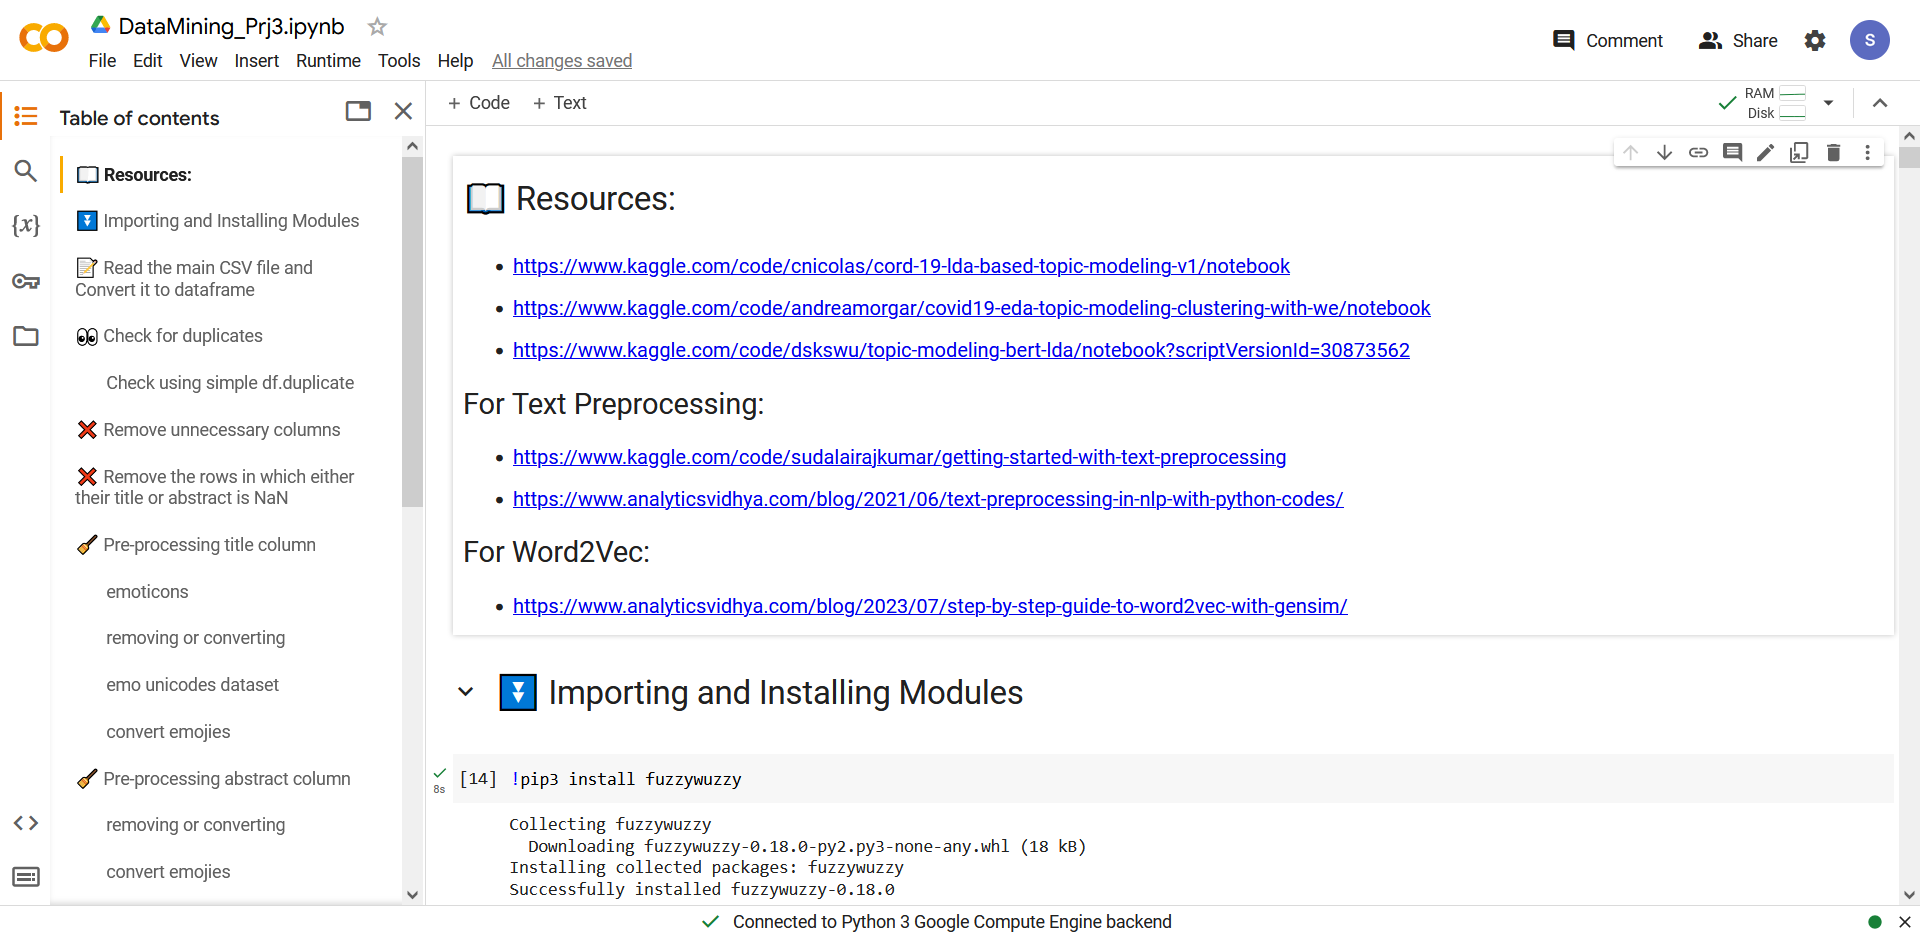
\includegraphics[width=0.8\textwidth]{step-1-colab-env.png}
        \caption{نمای کلی از پروژه \lr{notebook} در فضای \lr{Google Colab}}
        \label{fig:fig1}
    \end{figure}
    
در مرحله اول بااستفاده از کتابخانه \lr{pandas} و تابع \lr{read\_csv}، فایل ورودی را به آبجکتی از نوع \lr{dataframe} تبدیل می‌کنیم تا در قدم‌های بعدی راحت‌تر بتوانیم تحلیل‌های مورد نیاز را انجام بدهیم.
همچنین بااستفاده از توابع \lr{info()}، \lr{.head()} و \lr{.describe()} اطلاعات بیشتری نسبت به داده‌های موجود کسب می‌کنیم.

\begin{figure}[ht]
        \centering
        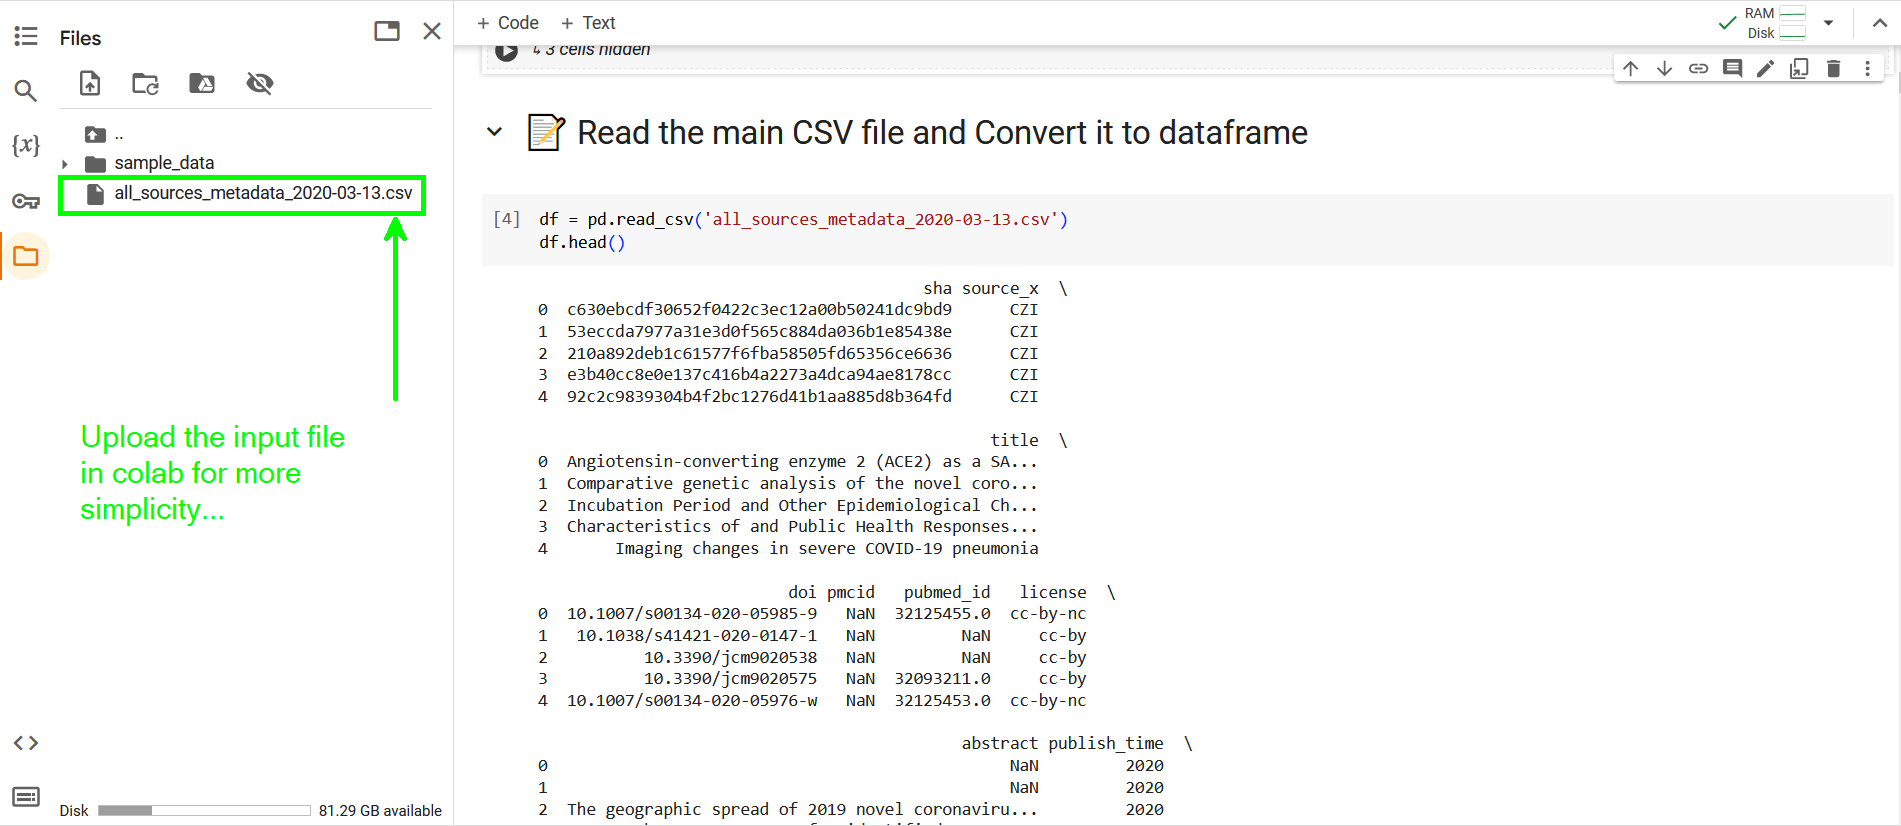
\includegraphics[width=0.8\textwidth]{step-1-read-csv.png}
        \caption{خواندن فایل ورودی}
        \label{fig:fig2}
    \end{figure}
\newpage
همچنین در بخش زیر می‌توانید خروجی مربوط به تابع \lr{.info()} را مشاهده کنید. همانطور که مشاهده می‌کنید، در هر ستون تعدادی مقادیر تهی یا به اصطلاح \lr{NaN} موجود است، که در گام بعدی مورد پردازش قرار می‌گیرند.
\lr{\lstinputlisting[frame=single,
    numbers=left,
    style=Python,
    showstringspaces=false,
    basicstyle=\ttfamily,
    backgroundcolor=\color{gray!20!white},
    breaklines=true]{step1.py}}


\newpage
\section{گام دوم}
در این مرحله که مربوط به پیش‌پردازش داده‌ها می‌باشد، باتوجه به این موضوع که داده‌هایی که در اختیار داریم از نوع متنی می‌باشند، نیاز است بعضی از پیش‌پردازش‌های معمول را اجرا کنیم. بطور خلاصه مراحل زیر برروی داده‌های انجام شده‌اند:

- حذف ردیف‌های تکراری: براساس جفت عنوان و خلاصه مقاله، داده‌های تکراری شناخته و پیدا شده‌اند و تنها آخرین نمونه تکراری از هر گروه برای ادامه مراحل باقی می‌ماند.

- حذف تمامی ستون‌ها به‌جز ستون‌های \lr{title} و \lr{abstract}

- حذف تمامی ردیف‌هایی که حداقل یکی از مقادیر \lr{title} یا \lr{abstract} در آن‌ها تهی می‌باشد.

- تبدیل محتوای ستون \lr{title} و \lr{abstract} به \lr{string}

- تبدیل تمامی حروف موجود در ستون‌های \lr{title} و \lr{abstract} به حروف کوچک

- حذف تمامی علائم نگارشی از ستون‌های \lr{title} و \lr{abstract}

- حذف برخی از حروف پرتکرار مانند \lr{for}، \lr{must} و ... از ستون‌های \lr{title} و \lr{abstract}

- برگرداندن کلمات موجود در ستون‌های \lr{title} و \lr{abstract} به ریشه اصلی آن‌ها با استفاده از عملیات \lr{stemming} و \lr{lemmatization}

- حذف \lr{emoticons} از محتوای ستون‌های \lr{title} و \lr{abstract}

- حذف آدرس‌ها از محتوای ستون‌های \lr{title} و \lr{abstract}

- حذف تگ‌های \lr{html} از محتوای ستون‌های \lr{title} و \lr{abstract}

- حذف برخی از رشته‌های خلاصه‌شده خاص از محتوای ستون‌های \lr{title} و \lr{abstract}

* خروجی تمامی مراحل بالا در دو ستون جدا به‌ نام‌های \lr{cleaned\_title} و \lr{cleaned\_abstract} و در آبجکت \lr{df\_dropped} ذخیره می‌شوند.

\newpage
\section{گام سوم}
این مرحله مربوط به استخراج ویژگی از داده‌های موجود می‌باشد. در این مرحله باتوجه به داده‌های متنی که در اختیار داریم، نیاز است تا برای پردازش راحت‌تر، کلمات را به مقادیر عددی تبدیل کنیم که برای انجام این کار از دو روش \lr{TF-IDF} و \lr{Bag of Words} استفاده شده‌است.
همچنین باتوجه به این موضوع که از ما خواسته‌شده است که تحلیل‌ها را بر روی دو ستون \lr{title} و \lr{abstract} انجام دهیم، درواقع مقادیر تجمیع شده این دو ستون را به‌عنوان ورودی به دو تابع \lr{TfidfVectorizer} و \lr{CountVectorizer} به‌عنوان ورودی می‌دهیم. این دو تابع در کتابخانه \lr{sklearn.feature\_extraction.text} موجود می‌باشند. و نحوه استفاده از این دو تابع را در کدهای زیر می‌توانید مشاهده کنید:

\lr{\lstinputlisting[frame=single,
    numbers=left,
    style=Python,
    showstringspaces=false,
    basicstyle=\ttfamily,
    backgroundcolor=\color{gray!20!white},
    breaklines=true]{step3.py}}

\newpage
\section{گام چهارم}
در این مرحله به‌منظور انجام \lr{Topic Modeling} از الگوریتم \lr{Latent Dirichlet Allocation} استفاده می‌کنیم. این الگوریتم را به‌طور مجزا یک بار با استفاده از ماتریس خروجی از الگوریتم \lr{TF-IDF} انجام می‌دهیم و بار دیگر نیز الگوریتم را برروی خروجی \lr{Bag of Words} اجرا می‌کنیم.
\begin{figure}[ht]
        \centering
        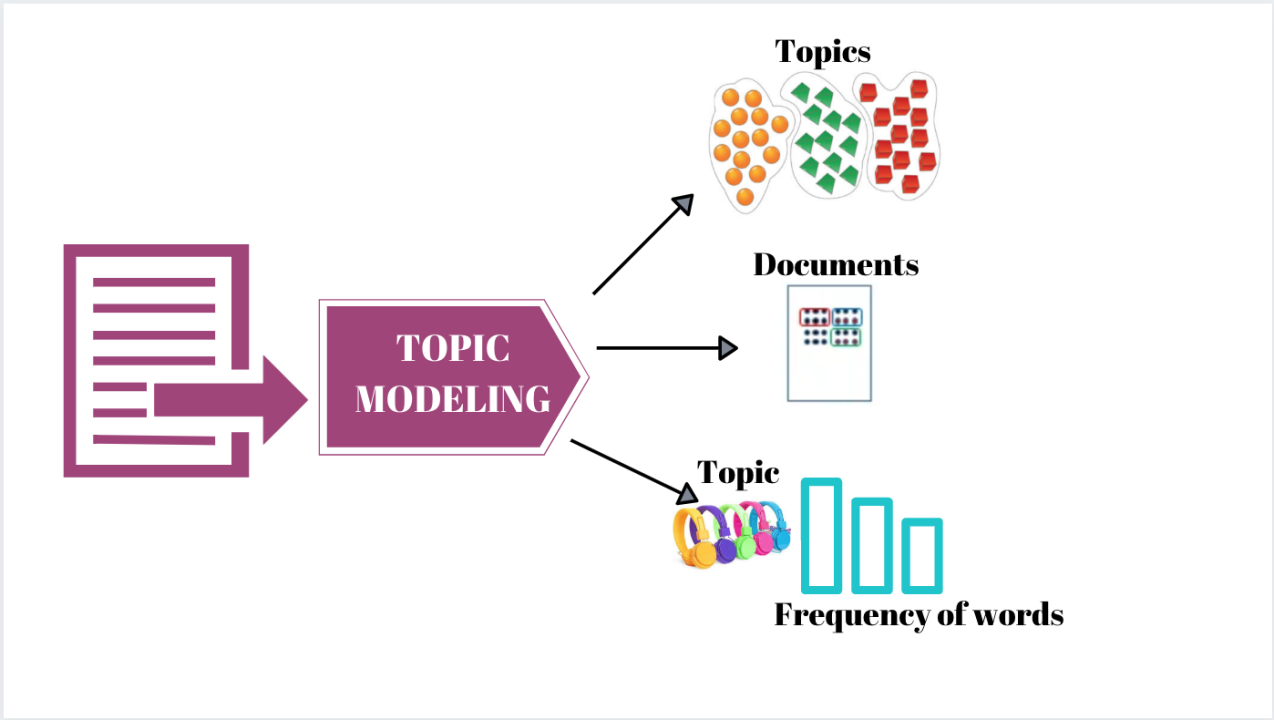
\includegraphics[width=0.7\textwidth]{step4-lda.png}
        \caption{الگوریتم \lr{LDA}}
        \label{fig:fig3}
\end{figure}

کدهای مربوط به این بخش را در بخش زیر می‌توانید مشاهده کنید:
\lr{\lstinputlisting[frame=single,
    numbers=left,
    style=Python,
    showstringspaces=false,
    basicstyle=\ttfamily,
    backgroundcolor=\color{gray!20!white},
    breaklines=true]{step4.py}}
    
\newpage
\section{گام پنجم}
در این مرحله از ما خواسته‌شده است تا ابعاد ماتریس‌هایی که در مرحله قبلی محاسبه شده بودند را کاهش دهیم. به‌منظور انجام این کار از الگوریتم \lr{Principle Component Analysis} استفاده می‌کنیم. در هنگام استفاده از این الگوریتم همانگونه که در تصویر زیر مشاهده می‌کنیم، تعداد بخش‌های اصلی را با 2 مقداردهی می‌کنیم. همانند مرحله پیشین نیاز است یک بار الگوریتم را با استفاده از ماتریس خروجی \lr{TF-IDF} و بار دیگر با استفاده از ماتریس خروجی \lr{Bag of Words} اجرا نمائیم.
\begin{figure}[ht]
        \centering
        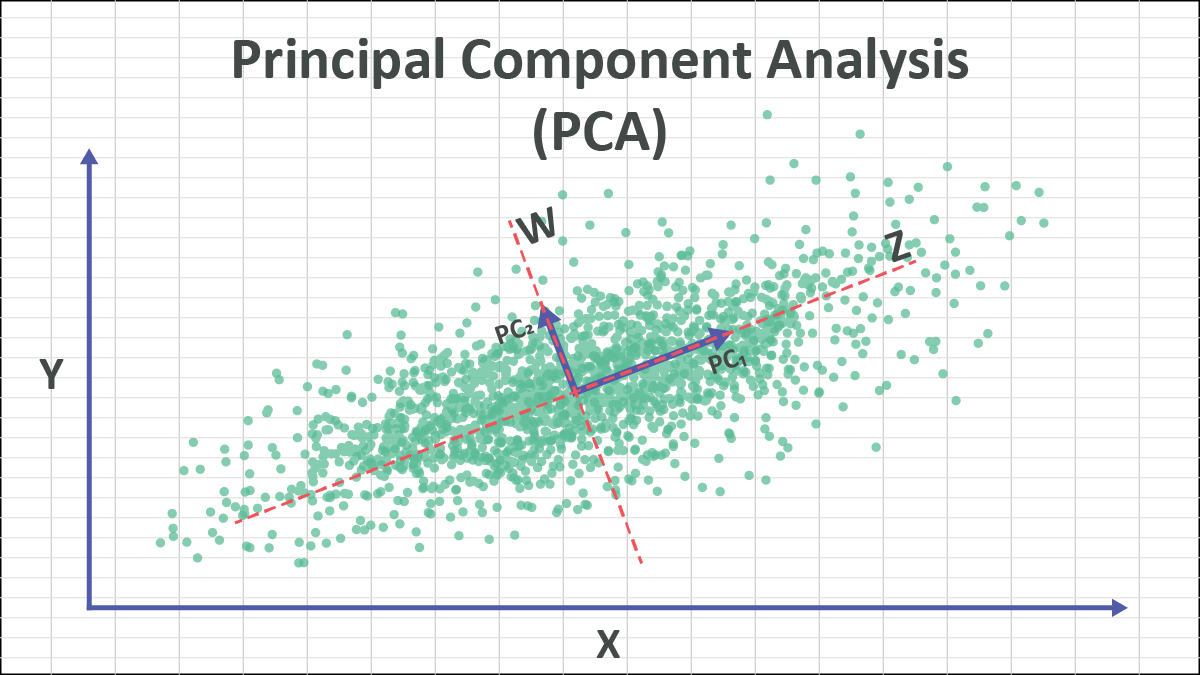
\includegraphics[width=0.7\textwidth]{step5-pca.png}
        \caption{الگوریتم \lr{PCA}}
        \label{fig:fig4}
\end{figure}

کدهای مربوط به این بخش را در بخش زیر می‌توانید مشاهده کنید:
\lr{\lstinputlisting[frame=single,
    numbers=left,
    style=Python,
    showstringspaces=false,
    basicstyle=\ttfamily,
    backgroundcolor=\color{gray!20!white},
    breaklines=true]{step5.py}}

\newpage
همچنین تصاویر مربوط به خروجی این الگوریتم را برروی دو ماتریس \lr{TF-IDF} و \lr{Bag of Words} می‌توانید مشاهده کنید:
\begin{figure}[ht]
        \centering
        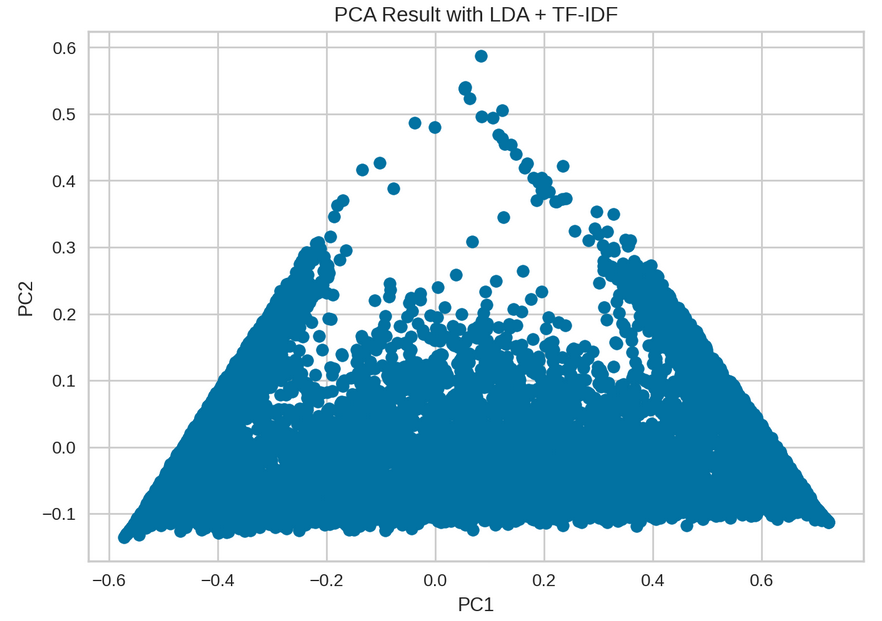
\includegraphics[width=0.5\textwidth]{step5-pca-tf-idf.png}
        \caption{خروجی الگوریتم \lr{PCA} برای ماتریس ورودی \lr{TF-IDF}}
        \label{fig:fig5}
\end{figure}

\begin{figure}[ht]
        \centering
        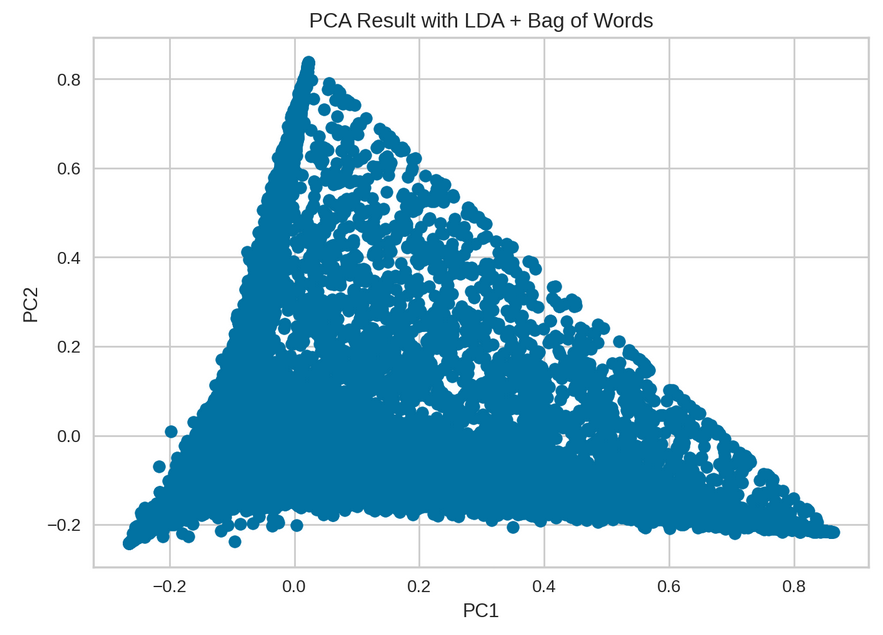
\includegraphics[width=0.5\textwidth]{step5-pca-bow.png}
        \caption{خروجی الگوریتم \lr{PCA} برای ماتریس ورودی \lr{BoW}}
        \label{fig:fig6}
\end{figure}

\newpage
\section{گام ششم}
در این مرحله که مربوط به استفاده از الگوریتم‌های خوشه‌بندی می‌باشد، همانطور که در تصویر زیر مشاهده می‌کنید از دو الگوریتم \lr{KMeans} و \lr{DBSCAN} استفاده می‌کنیم. البته هر یک از این دو الگوریتم را بصورت جداگانه بااستفاده از دو ماتریس \lr{TF-IDF} و \lr{Bag of Words} مورد آموزش قرار می‌دهیم.
همچنین هنگام استفاده از الگوریتم \lr{KMeans} بااستفاده از الگوریتم \lr{Elbow} و \lr{Silhoute} سعی می‌کنیم تا بهترین مقدار \lr{K} یا به‌عبارتی بهینه‌ترین تعداد خوشه‌ها را انتخاب کنیم. مقدار بازه تعداد خوشه‌ها را از 2 تا 20 تعریف می‌کنیم و همانطور که در خروجی مشخص است، در هر دو حالت تعداد خوشه دو بهترین پاسخ را باتوجه به معیار \lr{Silhoute} می‌دهد. چراکه همانطور که می‌دانیم هر چه مقدار این معیار به 1 نزدیک‌تر باشد، یعنی خوشه‌بندی بهتر انجام شده‌است. 
\begin{figure}[ht]
        \centering
        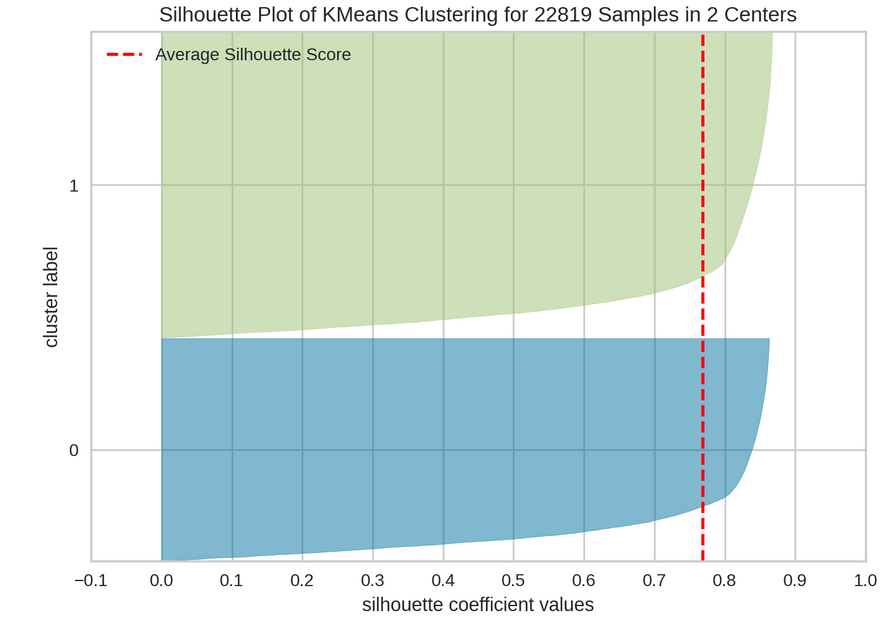
\includegraphics[width=0.5\textwidth]{step-6-sil-kmeans-tfidf.png}
        \caption{خروجی تابع \lr{Silhoute} برای الگوریتم \lr{KMeans} در حالت استفاده از الگوریتم \lr{TF-IDF}}
        \label{fig:fig7}
\end{figure}

\begin{figure}[ht]
        \centering
        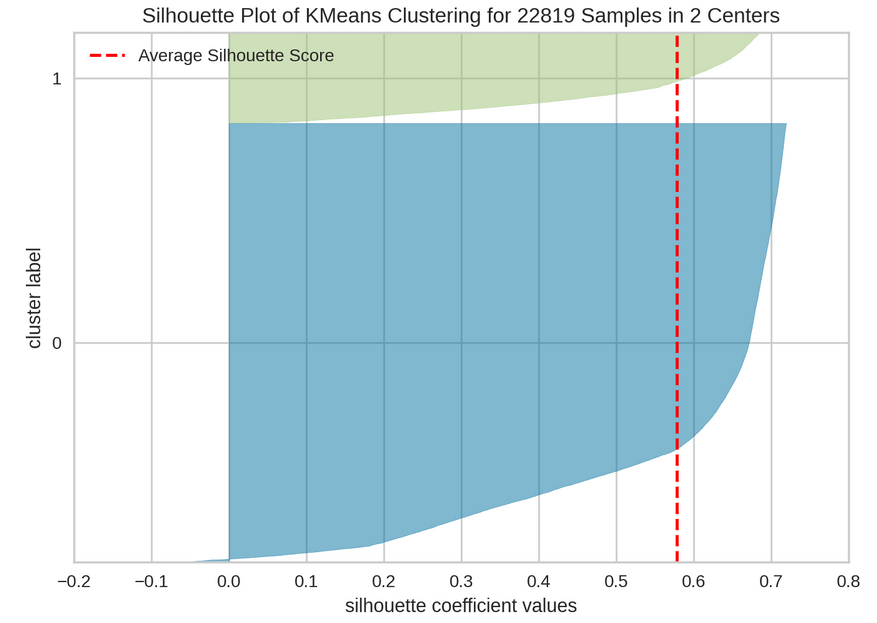
\includegraphics[width=0.5\textwidth]{step-6-sil-kmeans-bow.png}
        \caption{خروجی تابع \lr{Silhoute} برای الگوریتم \lr{KMeans} در حالت استفاده از الگوریتم \lr{Bag of Words}}
        \label{fig:fig8}
\end{figure}

\newpage
نمودارهای \lr{Elbow} مربوط به الگوریتم‌های \lr{KMeans} را نیز می‌توانید در تصاویر زیر مشاهده کنید:
\begin{figure}[ht]
        \centering
        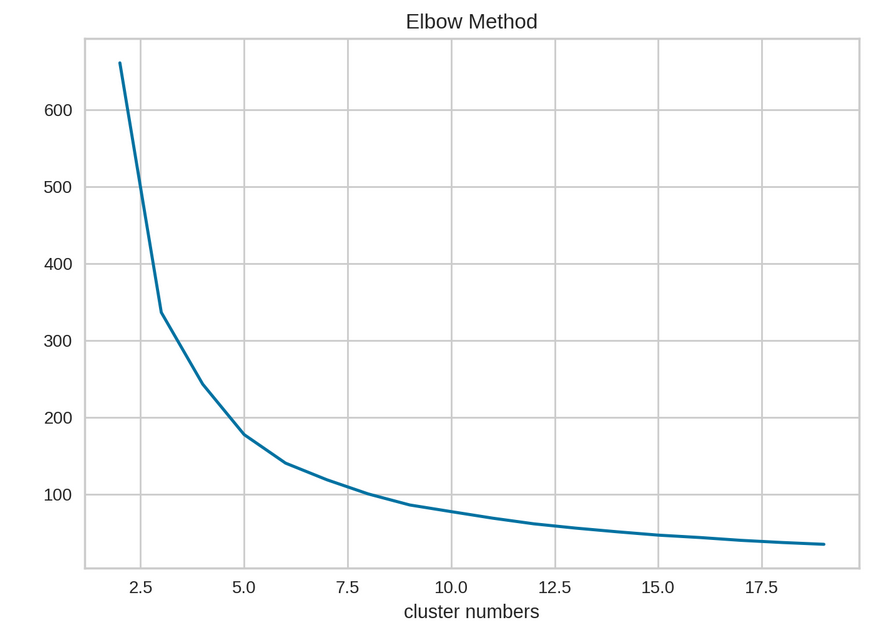
\includegraphics[width=0.5\textwidth]{kmeans-tfidf-elbow.png}
        \caption{\lr{Elbow for KMeans TF-IDF}}
        \label{fig:fig10}
\end{figure}

\begin{figure}[ht]
        \centering
        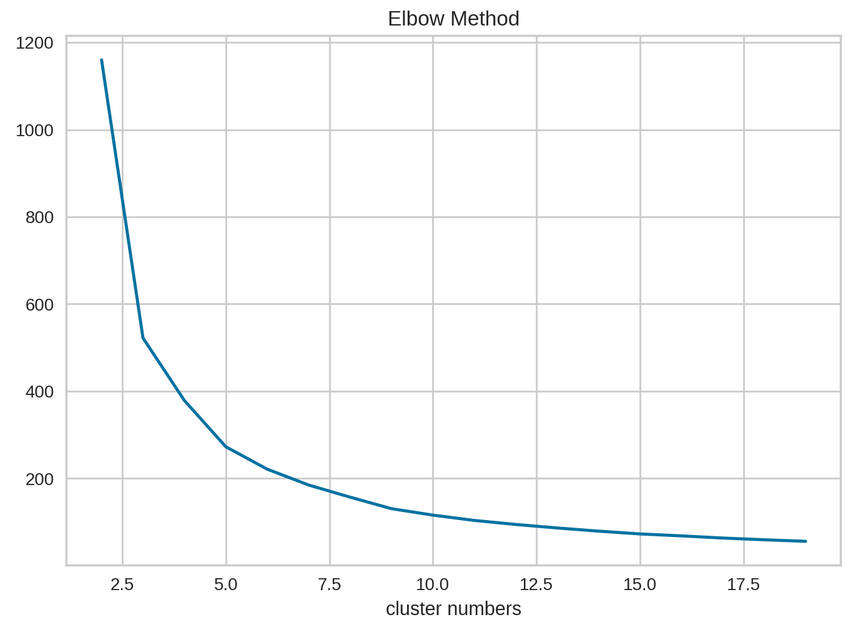
\includegraphics[width=0.5\textwidth]{kmeans-bow-elbow.png}
        \caption{\lr{Elbow for KMeans BoW}}
        \label{fig:fig11}
\end{figure}
*تمامی خروجی‌های مربوط به این بخش در خروجی کدها موجود است.

\newpage
\section{نتیجه‌گیری}
\subsection{کدام یک از روش استخراج ویژگی و مدل خوشه‌بندی عملکرد بهتری دارند؟}
در حالت استفاده از الگوریتم \lr{KMeans} و ماتریس نتایج \lr{TF-IDF} به‌همراه \lr{K=2} به بهترین عملکرد می‌رسیم.
\subsection{دلیل خود برای این انتخاب را ذکر کنید.}
سادگی پیاده‌سازی - قابلیت فهم بیشتر الگوریتم و نحوه عملکرد - کمبود زمان:)
\newpage
\subsection{با بررسی خوشه ها تحلیل کنید که هر خوشه نماینده ی کدام نوع از موضوعات می باشند.}
همانطور که در بخش زیر می‌توانید مشاهده کنید، ده عنوان پرتکرار در حالتی که تنها دو خوشه داشته باشیم، به‌صورت زیر می‌باشند:
\lr{\lstinputlisting[frame=single,
    numbers=left,
    style=Python,
    showstringspaces=false,
    basicstyle=\ttfamily,
    backgroundcolor=\color{gray!20!white},
    breaklines=true]{eval.py}}

\subsection{نمایش داده‌ها}
تصویر مربوط به خروجی الگوریتم \lr{KMeans} را با دو خوشه می‌توانید در تصویر زیر مشاهده کنید.
باتوجه به اینکه پیش از استفاده از خوشه‌بندی، از الگوریتم کاهش ابعاد استفاده کردیم، دقت مدل متاسفانه کاهش یافته است و به این دلیل که داده‌ها را به دو بعد کاهش داده‌ایم، امکان دارد که بعد دوم در زیر این بعد قرار داشته باشد.

* سایر نمایش‌های مربوط به خوشه‌ها در خروجی برنامه قرار دارند.
\begin{figure}[ht]
        \centering
        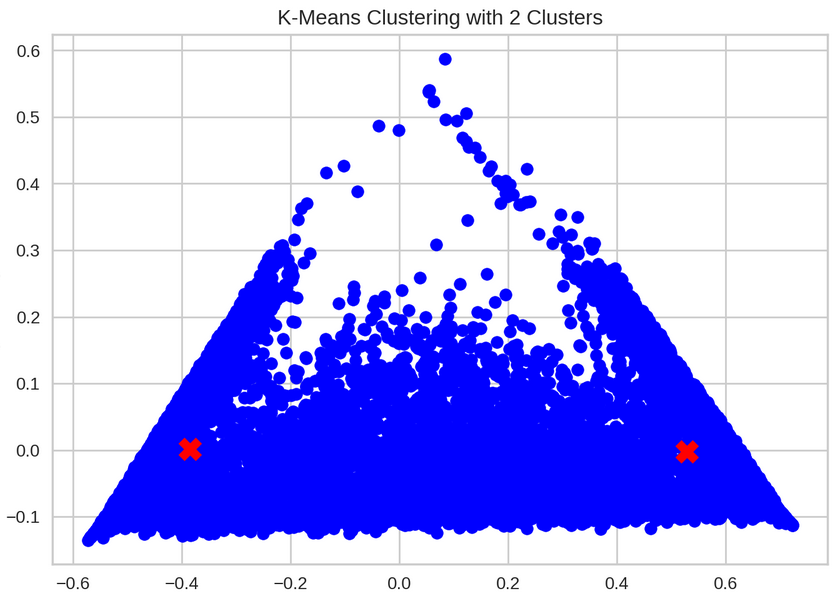
\includegraphics[width=0.5\textwidth]{eval-vis.png}
        \caption{\lr{Clustering Visualize}}
        \label{fig:fig9}
\end{figure}
\end{document}
